\documentclass[11pt]{article}
\usepackage{graphicx}
%Gummi|065|=)
\title{\textbf{Conductivity Estimation}}
\author{Ivan Viti}
\date{March 24}
\begin{document}

\maketitle

\section{Calculate conductivity}

\begin{eqnarray}
\sigma = \frac{2} {\hbar} e^2 a^{2-d} g \exp(-\sqrt{T_o / T})
\label{conductanceGlatz}
\end{eqnarray}

	where $\hbar$ is Plank's constant, $e$ is the charge of an electron, $g = .1$ is the intergrain conductance, $T_o$ is the characteristic temperature scale (energy required to stack 2 electrons on the same site (1600 Kelvin in our case) ). The next step is to define conductance so that it can be found in terms of Dias parameters.
	
 \begin{eqnarray}
\sigma = \frac{J} {E} = \frac {A \cdot m^{-1}} {V \cdot m^{-1}} 
\label{conductanceWiki}
\end{eqnarray}

where $J$ (current density) is coulombs per second per meter and $E$ (electric field) is joules per coulomb per meter. In my simulation, I deal with individual electrons and smaller scale. Electrons per second per 15 nm are converted to coulombs per second per meter. Converting the top gives

\begin{eqnarray}
J = \frac {e} {15nm \cdot s} = \frac{ 1.6\times 10^{-19} C} {1.5\times 10^{-8} m \cdot s}  , 
\label{convertJ}
\end{eqnarray}
which gives a conversion factor $\approx 1.06 \times 10^{-11} $.

\section{Calculate inverse escape rate}
Next, we need the inverse escape rate prefactor. This is defined as
\begin{eqnarray}
\Gamma = \tau^{-1} = g \delta 
\label{escapeRate}
\end{eqnarray}
where $\delta$ is the mean energy level spacing. For our 15 nm grain, $\delta \approx 1 meV$, $g = .1$. Then we have $\Gamma = .1 meV$. We divide by $\hbar$ to get units of time. This gives us an escape rate prefactor of $\tau = 6.5\times 10^{10}$ 

The escape rate $\tau^{-1}$ is used to pull time from the sum of the probabilities. The electric field is set to 0.001 volts per meter.  

 \begin{figure}[htbp]
\begin{center}
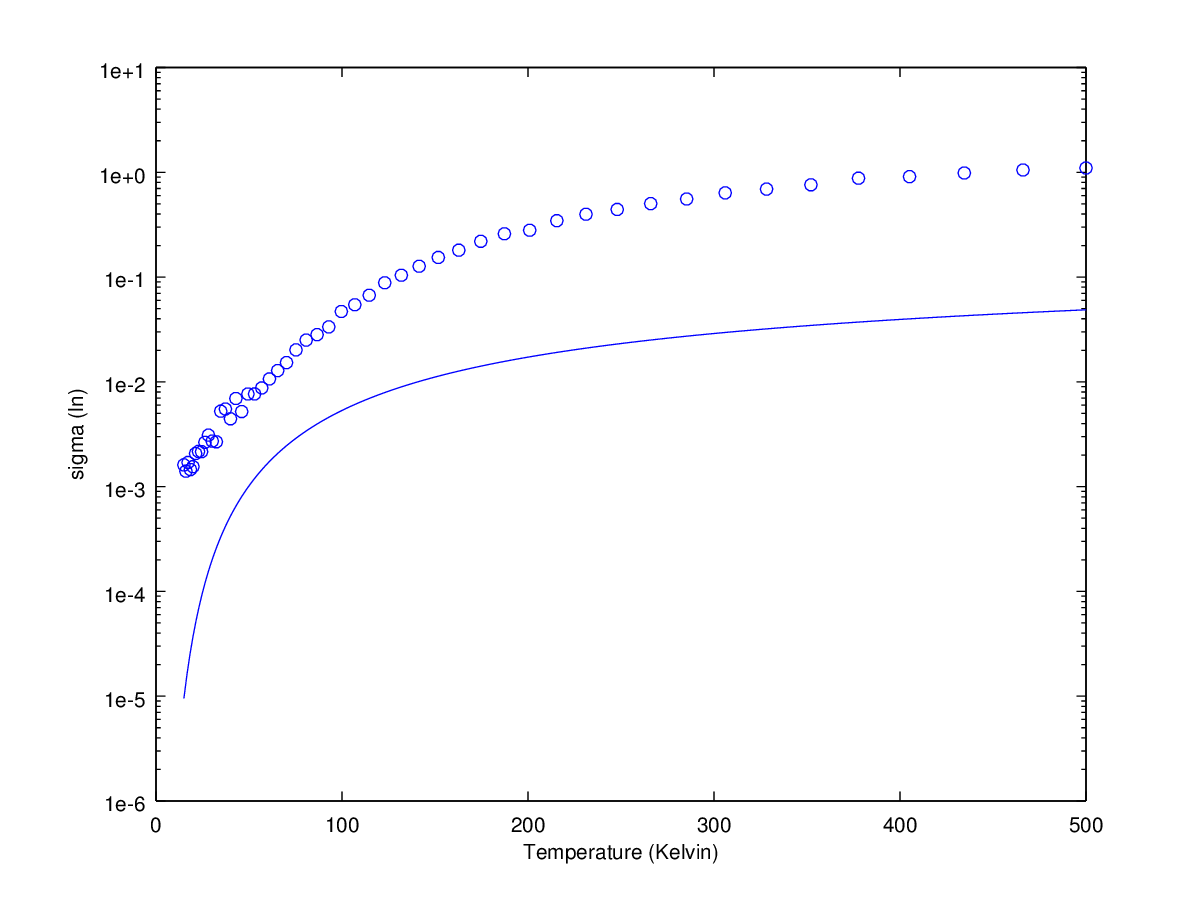
\includegraphics[scale=.50]{TvSigUnits.png}
\caption{Temperature vs Conductivity. Solid line is analytic while dots are simulated.}
\label{TvSig}
\end{center}
\end{figure}

\end{document}
